\section{Speicher Management}\label{sec:speicherman}
Der Speicher ist ganz klar die wichtigste Komponente beim schreiben von einem Programm, denn ohne
den Speicher geht nichts. Da diese Komponente so enorm wichtig ist, muss auch besonders darauf
acht gegeben werden. Vor allem wenn es um die Performance eines Programms geht, kann beim
Speicher Management viel herausgeholt werden. In C++ ist dem Programmierer die Möglichkeit
gegeben, zwischen dem \emph{Stack} und dem \emph{Heap} zu Entscheiden, wo dieser seine Objekte
speichert.

\subsection{Stack}
Dabei ist die Speicherung auf dem \emph{Stack} aus Performanter Sicht sehr lukrativ, da dass
Speichern und Verwerfen von Objekten sehr schnell von statten gehen kann. Jedoch ist nichts
umsonst und der \emph{Stack} kommt mit einigen Einschränkungen wie zum Beispiel der festen Größe,
die in Embedded Systems nicht besonders groß sein muss, oder auch das keine Dynamischen Objekte
dort gespeichert werden können \cite{C++HighPer2}.

\subsection{Heap}
Sollen Objekte nun Dynamisch gespeichert werden, dann kommt der Programmierer nicht drum herum,
diese Objekte auf dem \emph{Heap} abzulegen. Dies kann erreicht werden, mit der Verwendung von
der Funktion \emph{malloc} oder mit dem C++ Operator \emph{new}. Im Endeffekt wird \emph{malloc}
im \emph{new} Operator aufgerufen, der einzige Unterschied zwischen \emph{malloc} und \emph{new}
ist, das bei \emph{new} noch der Konstruktor des Objektes aufgerufen wird. Das große Problem,
welches entsteht bei der Verwendung vom \emph{Heap}, ist dass diese Operation sehr teuer aus
Performanter Sicht ist. Zwei Faktoren weshalb diese Operation so teuer ist spielen dabei eine
Rolle. Zum einen ist das Anfordern von frischem Speicher an sich eine sehr teure Angelegenheit
und zum anderen ist die Platzierung der Daten komplett willkürlich, was zu sogenannten
\emph{cache misses} führen kann.
\newline
\newline
\emph{Cach misses} sind unter anderem sehr kostspielig wenn es um Mehrdimensionale Arrays geht.
Im folgenden wird als Beispiel ein Dynamisches zweidimensionales Array auf dem \emph{Heap} abgelegt:

\begin{lstlisting}[
    caption={Anlegen eines Zweidimensionalem Array auf dem Heap},
    label=lst:Heap2DArray,
    language=C++,frame=tlrb]
int main(int argc, char** argv){
	int** array2d = new int*[5];
	for (int i = 0; i < 5; ++i)
		array2d[i] = new int[5];
}
\end{lstlisting}

Nachdem das Array angelegt wurde, hat der Programmierer die Möglichkeit sich die Adressen
anzusehen, wie im Folgenden durch eine Konsolen Ausgabe.

\begin{lstlisting}[
    caption={Mögliche Ausgabe der Adressen},
    label=lst:ArrayAdressen,
    language=C++]
arr2d[0]: 010B5188
arr2d[1]: 010B51C8
arr2d[2]: 010B52C8
arr2d[3]: 010B5308
arr2d[4]: 010BEE78
\end{lstlisting}

Zu sehen ist, dass die Adressen sehr weit auseinander liegen, was dann sehr Langsam sein kann
wenn das Array beschrieben werden soll.

\subsection{Speicher auf dem Heap zuweisen}
Wie schon vorher erwähnt sind die \emph{cach misses} nicht die einzigen Performance Probleme, die
entstehen wenn Objekte auf dem \emph{Heap} gespeichert werden. Um Speicher vom \emph{Heap} zu
bekommen, muss der \emph{memory allocator} folgende Anforderungen erfüllen:

\begin{itemize}
    \item Es muss \emph{Multithreading} Unterstützen, da alle Threads nur auf den globalen
    \item \emph{Heap} zugreifen, daher muss es auch eine Art von Synchronisation implementiert
    \item haben.
    \item Es muss effizient verschiedene Größen von Objekten zuweisen können.
    \item Es sollte sich nicht über die Zeit verschlechtern.
    \item Am Anfang eines Programm wird vom Betriebssystem dem Programm speicher zur Verfügung
    \item gestellt und wenn dieser Aufgebraucht ist, dann muss es runter zum \emph{kernel} um
    \item neuen Speicher anzufordern.
\end{itemize}

All diese Anforderungen und noch einige mehr müssen erfüllt werden! Zu sehen ist also, dass das
Speicher auf dem \emph{Heap} keines falls Trivial ist und mit bedacht einzusetzen ist
\cite{HandsOn}[vgl.].

\subsection{Benchmarking Stack vs. Heap}
Theorie ist gut, Praxis ist besser! Nach diesem Motto soll in dieser Sektion zwischen den beiden
Speicher Möglichkeiten, verglichen werden, wie groß der Performance Unterschied tatsächlich ist.
Für diesen Zweck wurde ein Zweidimensionales Array der Größe \emph{10x10} sowohl auf dem
\emph{Stack}, als auch auf dem \emph{Heap} gespeichert und dessen Felder auf den Wert 2 gesetzt.
Dabei wurde die Compiler Optimierung ausgestellt, damit nichts essentielles vom Compiler bei
diesem Versuch wegoptimiert wird. Dieser Vorgang wurde dann \emph{N} Mal wiederholt und
resultierte in das folgende Ergebnis:

\begin{figure}[h]
    \centering
    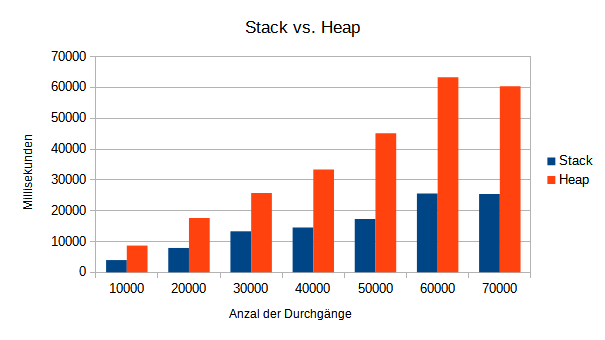
\includegraphics[width=0.5\textwidth]{bilder/StackvsHeap}
    \caption[StackvsHeap]{\emph{Stack} vs. \emph{Heap}}
    \label{img:StackvsHeap}
\end{figure}

Wie zu sehen ist, ist die \emph{Heap} Speicherung deutlich langsamer und der Performance
unterschied ist keinesfalls zu Unterschätzen.
\newline
\newline
Ein Interessanter Fakt der zudem noch zu beobachten war, war dass der Compiler auf der höchsten
Compiler Optimierungsstufe, in der Lage war, den Stack Code wegzuoptimieren. Dadurch wurde der
Komplette Code für die Stack Implementierung verworfen und die gemessene Zeit resultierte in 0
Mikrosekunden.

\subsection{New Operator Überschreiben}
\begin{zitat}
    If we need dynamic memory and can't avoid allocations, we may have to write a custom memory
    manager that performs better for our specific needs \cite{C++HighPer2}.
\end{zitat}
In der Vorhergehenden Sektion wurde für das Speichern auf dem \emph{Heap} die Standard Implementation von C
beziehungsweise C++ benutzt, dies ist jedoch nur eine generelle Funktion zum Zuweisen von
Speicher, deswegen auch auf nichts spezialisiert. C++ bietet dem Programmierer die Möglichkeit
seine eigene Implementation zu schreiben, indem der \emph{new} Operator Überschrieben wird. Zum
Beispiel könnte am Anfang des Programms einmalig der gesamte Speicher, welches das ungefähr
Programm braucht reserviert werden, um dann vom reservierten Speicher alle Objekte zu verwalten.
\newline
\newline
Neben der eigen Implementierung existieren natürlich noch externe alternativen zu der Standard
Implementierung von \emph{malloc}, wie zum Beispiel die Implementierung von Google, welche die
\emph{tcmalloc} Funktion zur Verfügung stellen.

\subsection{Zusammenfassung}
Abschließend kann gesagt werden, dass Speicher vom \emph{Heap} extrem kostspielig ist und hinter
dem \emph{new} Operator mehr steckt als manch einer vielleicht vermutet. Wie zudem auch zu sehen
war, ist die Möglichkeit gegeben, eine eigene Implementierung zu schreiben oder auf externe
Implementierungen zurückzugreifen. Alles im allem bleibt die Benutzung des \emph{Heap} sehr teuer
und es sollte wann immer möglich mit dem \emph{Stack} gearbeitet werden.